\documentclass{beamer}
\usepackage{graphicx} % Required for inserting images

\title{Verifica funzionale di programmi con Dafny}
\author{Lorenzo Quellerba}
\institute{Univeristà degli Studi di Torino}
\date{June 2023}

\begin{document}
\maketitle

\begin{frame}{Verifica funzionale}
    Qua dentro accenni al problema della verifica funzionale (letteralmente al massimo la tripla di Hoare e i predicate transformer)
\end{frame}

\begin{frame}{Dafny}
    Qua parli di Dafny
\end{frame}

\begin{frame}{Albero binario di ricerca}
    Implementazione dell'albero binario di ricerca
\end{frame}

\begin{frame}{Il rene}
    \begin{enumerate}
        \item Il rene è un organo del corpo umano
        \item È molto importante
        \item Non puoi vivere senza entrambi ma con solo uno si
    \end{enumerate}
    \begin{figure}
        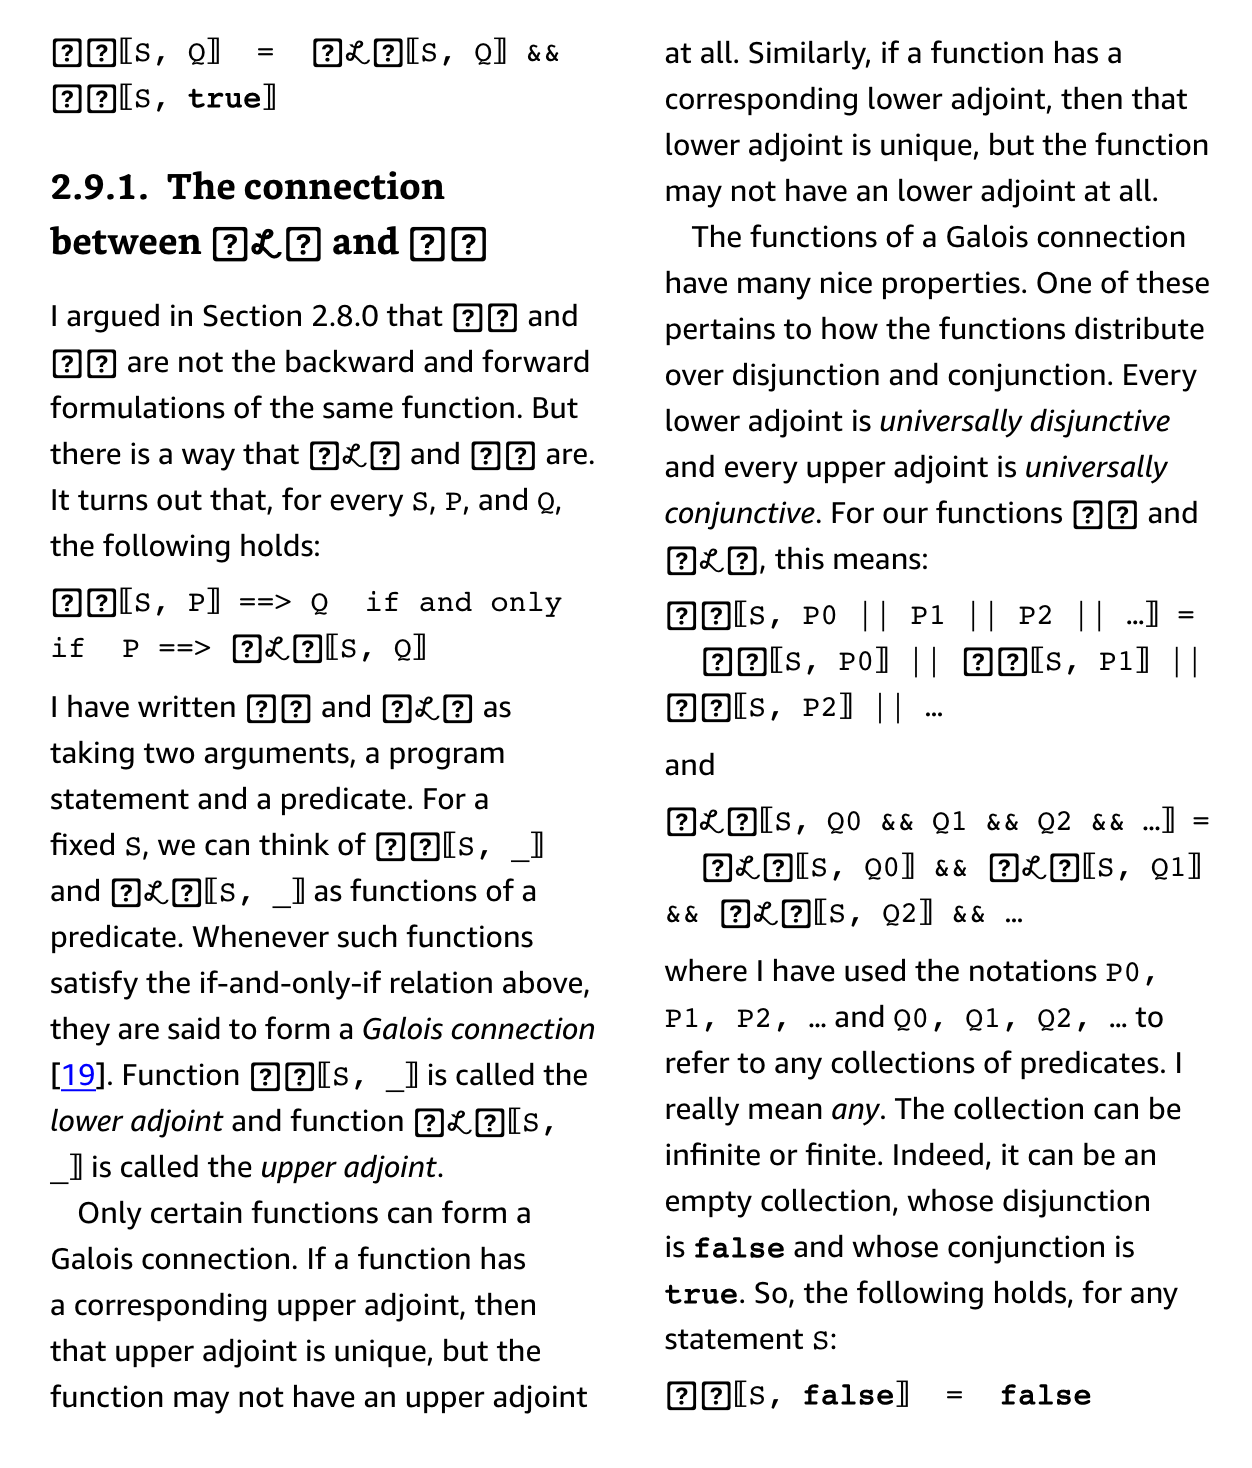
\includegraphics[scale=0.4]{Screenshot 2023-06-01 at 14.25.40.png}
    \end{figure}
\end{frame}

\begin{frame}
    \begin{enumerate}
        \onslide<1-> \item Primo elemento
        \onslide<2-> \item Secondo elemento
        \onslide<3->  \item Terzo elemento
        \onslide<4>  \item Quarto elemento
    \end{enumerate}
\end{frame}

\begin{frame}
    \only<1>{Ciao}
    \only<2>{Mondo}
\end{frame}

\begin{frame}{Titolo della slide}
    \begin{enumerate}
        \only<1->{
            \item Vorrei questo nella prima
            \item Anche questo nella prima
        }
        \only<2>{
            \item Questo nella seconda
            \item Questo nella seconda
        }
    \end{enumerate}
\end{frame}

\end{document}
